% Created by tikzDevice version 0.10.1 on 2018-01-31 10:28:54
% !TEX encoding = UTF-8 Unicode
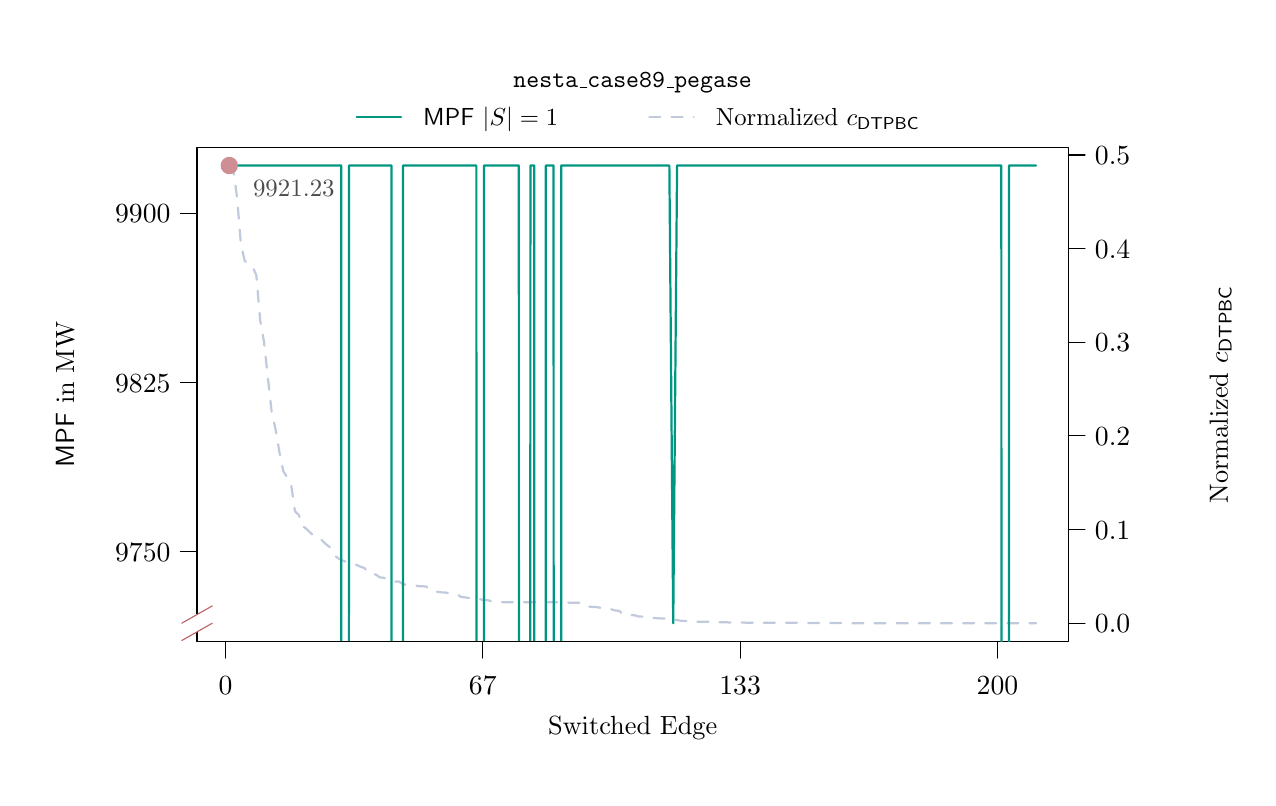
\begin{tikzpicture}[x=1pt,y=1pt]
\definecolor{fillColor}{RGB}{255,255,255}
\path[use as bounding box,fill=fillColor,fill opacity=0.00] (0,0) rectangle (440.85,271.01);
\begin{scope}
\path[clip] (  0.00,  0.00) rectangle (440.85,271.01);
\definecolor{drawColor}{RGB}{193,202,220}

\path[draw=drawColor,line width= 0.8pt,dash pattern=on 4pt off 4pt ,line join=round,line cap=round] ( 72.86,221.20) --
	( 74.26,220.12) --
	( 75.65,209.79) --
	( 77.05,192.73) --
	( 78.44,186.68) --
	( 79.84,185.86) --
	( 81.23,184.60) --
	( 82.62,181.58) --
	( 84.02,165.25) --
	( 85.41,157.39) --
	( 86.81,144.42) --
	( 88.20,131.90) --
	( 89.60,125.76) --
	( 90.99,117.47) --
	( 92.39,110.68) --
	( 93.78,108.57) --
	( 95.18,106.06) --
	( 96.57, 96.25) --
	( 97.97, 94.96) --
	( 99.36, 90.98) --
	(100.76, 89.86) --
	(102.15, 88.52) --
	(103.55, 87.22) --
	(104.94, 86.71) --
	(106.34, 85.76) --
	(107.73, 84.42) --
	(109.13, 83.34) --
	(110.52, 80.70) --
	(111.92, 79.45) --
	(113.31, 78.67) --
	(114.71, 78.11) --
	(116.10, 77.55) --
	(117.50, 77.33) --
	(118.89, 76.86) --
	(120.29, 76.21) --
	(121.68, 75.78) --
	(123.08, 73.92) --
	(124.47, 73.74) --
	(125.87, 73.36) --
	(127.26, 72.36) --
	(128.66, 72.23) --
	(130.05, 71.50) --
	(131.44, 71.41) --
	(132.84, 70.85) --
	(134.23, 70.85) --
	(135.63, 69.90) --
	(137.02, 69.73) --
	(138.42, 69.60) --
	(139.81, 69.51) --
	(141.21, 69.21) --
	(142.60, 69.17) --
	(144.00, 69.04) --
	(145.39, 67.83) --
	(146.79, 67.31) --
	(148.18, 67.13) --
	(149.58, 66.96) --
	(150.97, 66.92) --
	(152.37, 66.62) --
	(153.76, 66.36) --
	(155.16, 66.31) --
	(156.55, 65.32) --
	(157.95, 65.15) --
	(159.34, 64.97) --
	(160.74, 64.80) --
	(162.13, 64.50) --
	(163.53, 64.46) --
	(164.92, 64.20) --
	(166.32, 64.11) --
	(167.71, 63.68) --
	(169.11, 63.64) --
	(170.50, 63.46) --
	(171.90, 63.42) --
	(173.29, 63.42) --
	(174.69, 63.42) --
	(176.08, 63.42) --
	(177.48, 63.42) --
	(178.87, 63.42) --
	(180.26, 63.42) --
	(181.66, 63.42) --
	(183.05, 63.42) --
	(184.45, 63.42) --
	(185.84, 63.42) --
	(187.24, 63.42) --
	(188.63, 63.42) --
	(190.03, 63.42) --
	(191.42, 63.42) --
	(192.82, 63.33) --
	(194.21, 63.33) --
	(195.61, 63.25) --
	(197.00, 63.20) --
	(198.40, 63.20) --
	(199.79, 63.16) --
	(201.19, 62.08) --
	(202.58, 61.86) --
	(203.98, 61.69) --
	(205.37, 61.65) --
	(206.77, 61.43) --
	(208.16, 61.26) --
	(209.56, 60.87) --
	(210.95, 60.83) --
	(212.35, 60.39) --
	(213.74, 60.31) --
	(215.14, 58.93) --
	(216.53, 58.71) --
	(217.93, 58.71) --
	(219.32, 58.67) --
	(220.72, 58.23) --
	(222.11, 58.19) --
	(223.51, 57.98) --
	(224.90, 57.85) --
	(226.30, 57.72) --
	(227.69, 57.59) --
	(229.08, 57.54) --
	(230.48, 57.50) --
	(231.87, 57.50) --
	(233.27, 57.20) --
	(234.66, 56.94) --
	(236.06, 56.68) --
	(237.45, 56.64) --
	(238.85, 56.46) --
	(240.24, 56.42) --
	(241.64, 56.38) --
	(243.03, 56.33) --
	(244.43, 56.33) --
	(245.82, 56.33) --
	(247.22, 56.25) --
	(248.61, 56.16) --
	(250.01, 56.16) --
	(251.40, 56.16) --
	(252.80, 56.12) --
	(254.19, 56.07) --
	(255.59, 56.07) --
	(256.98, 56.07) --
	(258.38, 56.07) --
	(259.77, 55.99) --
	(261.17, 55.99) --
	(262.56, 55.99) --
	(263.96, 55.99) --
	(265.35, 55.99) --
	(266.75, 55.99) --
	(268.14, 55.99) --
	(269.54, 55.99) --
	(270.93, 55.99) --
	(272.33, 55.99) --
	(273.72, 55.99) --
	(275.12, 55.99) --
	(276.51, 55.99) --
	(277.90, 55.94) --
	(279.30, 55.94) --
	(280.69, 55.94) --
	(282.09, 55.90) --
	(283.48, 55.90) --
	(284.88, 55.90) --
	(286.27, 55.90) --
	(287.67, 55.90) --
	(289.06, 55.90) --
	(290.46, 55.90) --
	(291.85, 55.90) --
	(293.25, 55.90) --
	(294.64, 55.90) --
	(296.04, 55.86) --
	(297.43, 55.82) --
	(298.83, 55.82) --
	(300.22, 55.82) --
	(301.62, 55.82) --
	(303.01, 55.82) --
	(304.41, 55.82) --
	(305.80, 55.82) --
	(307.20, 55.82) --
	(308.59, 55.82) --
	(309.99, 55.82) --
	(311.38, 55.82) --
	(312.78, 55.82) --
	(314.17, 55.82) --
	(315.57, 55.82) --
	(316.96, 55.82) --
	(318.36, 55.82) --
	(319.75, 55.82) --
	(321.15, 55.82) --
	(322.54, 55.82) --
	(323.94, 55.82) --
	(325.33, 55.82) --
	(326.72, 55.82) --
	(328.12, 55.82) --
	(329.51, 55.82) --
	(330.91, 55.82) --
	(332.30, 55.82) --
	(333.70, 55.82) --
	(335.09, 55.82) --
	(336.49, 55.82) --
	(337.88, 55.82) --
	(339.28, 55.82) --
	(340.67, 55.82) --
	(342.07, 55.82) --
	(343.46, 55.82) --
	(344.86, 55.82) --
	(346.25, 55.82) --
	(347.65, 55.82) --
	(349.04, 55.82) --
	(350.44, 55.82) --
	(351.83, 55.82) --
	(353.23, 55.82) --
	(354.62, 55.82) --
	(356.02, 55.82) --
	(357.41, 55.82) --
	(358.81, 55.82) --
	(360.20, 55.82) --
	(361.60, 55.82) --
	(362.99, 55.82) --
	(364.39, 55.82);
\end{scope}
\begin{scope}
\path[clip] (  0.00,  0.00) rectangle (440.85,271.01);
\definecolor{drawColor}{RGB}{0,0,0}

\path[draw=drawColor,line width= 0.4pt,line join=round,line cap=round] ( 61.20, 49.20) --
	(376.05, 49.20) --
	(376.05,227.81) --
	( 61.20,227.81) --
	( 61.20, 49.20);
\end{scope}
\begin{scope}
\path[clip] (  0.00,  0.00) rectangle (440.85,271.01);
\definecolor{drawColor}{RGB}{0,0,0}

\path[draw=drawColor,line width= 0.4pt,line join=round,line cap=round] (376.05, 55.82) -- (376.05,225.00);

\path[draw=drawColor,line width= 0.4pt,line join=round,line cap=round] (376.05, 55.82) -- (382.05, 55.82);

\path[draw=drawColor,line width= 0.4pt,line join=round,line cap=round] (376.05, 89.65) -- (382.05, 89.65);

\path[draw=drawColor,line width= 0.4pt,line join=round,line cap=round] (376.05,123.49) -- (382.05,123.49);

\path[draw=drawColor,line width= 0.4pt,line join=round,line cap=round] (376.05,157.33) -- (382.05,157.33);

\path[draw=drawColor,line width= 0.4pt,line join=round,line cap=round] (376.05,191.16) -- (382.05,191.16);

\path[draw=drawColor,line width= 0.4pt,line join=round,line cap=round] (376.05,225.00) -- (382.05,225.00);

\node[text=drawColor,anchor=base west,inner sep=0pt, outer sep=0pt, scale=  1.00] at (385.65, 52.37) {0.0};

\node[text=drawColor,anchor=base west,inner sep=0pt, outer sep=0pt, scale=  1.00] at (385.65, 86.21) {0.1};

\node[text=drawColor,anchor=base west,inner sep=0pt, outer sep=0pt, scale=  1.00] at (385.65,120.05) {0.2};

\node[text=drawColor,anchor=base west,inner sep=0pt, outer sep=0pt, scale=  1.00] at (385.65,153.88) {0.3};

\node[text=drawColor,anchor=base west,inner sep=0pt, outer sep=0pt, scale=  1.00] at (385.65,187.72) {0.4};

\node[text=drawColor,anchor=base west,inner sep=0pt, outer sep=0pt, scale=  1.00] at (385.65,221.56) {0.5};
\end{scope}
\begin{scope}
\path[clip] (  0.00,  0.00) rectangle (440.85,271.01);
\definecolor{drawColor}{RGB}{0,150,130}

\path[draw=drawColor,line width= 0.8pt,line join=round,line cap=round] (118.89,238.60) -- (134.91,238.60);
\definecolor{drawColor}{RGB}{193,202,220}

\path[draw=drawColor,line width= 0.8pt,dash pattern=on 4pt off 4pt ,line join=round,line cap=round] (224.63,238.60) -- (240.65,238.60);
\definecolor{drawColor}{RGB}{0,0,0}

\node[text=drawColor,anchor=base,inner sep=0pt, outer sep=0pt, scale=  0.89] at (218.62,249.28) {\texttt{nesta\_case89\_pegase}};

\node[text=drawColor,anchor=base west,inner sep=0pt, outer sep=0pt, scale=  0.89] at (142.92,235.54) {$\mathsf{MPF}~|S|=1$};

\node[text=drawColor,anchor=base west,inner sep=0pt, outer sep=0pt, scale=  0.89] at (248.66,235.54) {Normalized~$c_\mathsf{DTPBC}$};
\end{scope}
\begin{scope}
\path[clip] (  0.00,  0.00) rectangle (440.85,271.01);
\definecolor{drawColor}{RGB}{0,0,0}

\path[draw=drawColor,line width= 0.4pt,line join=round,line cap=round] ( 61.20, 81.70) -- ( 61.20,203.90);

\path[draw=drawColor,line width= 0.4pt,line join=round,line cap=round] ( 61.20, 81.70) -- ( 55.20, 81.70);

\path[draw=drawColor,line width= 0.4pt,line join=round,line cap=round] ( 61.20,142.80) -- ( 55.20,142.80);

\path[draw=drawColor,line width= 0.4pt,line join=round,line cap=round] ( 61.20,203.90) -- ( 55.20,203.90);

\node[text=drawColor,anchor=base east,inner sep=0pt, outer sep=0pt, scale=  1.00] at ( 51.60, 78.25) {9750};

\node[text=drawColor,anchor=base east,inner sep=0pt, outer sep=0pt, scale=  1.00] at ( 51.60,139.36) {9825};

\node[text=drawColor,anchor=base east,inner sep=0pt, outer sep=0pt, scale=  1.00] at ( 51.60,200.46) {9900};
\end{scope}
\begin{scope}
\path[clip] (  0.00,  0.00) rectangle (440.85,271.01);
\definecolor{drawColor}{RGB}{255,255,255}
\definecolor{fillColor}{RGB}{255,255,255}

\path[draw=drawColor,line width= 0.4pt,line join=round,line cap=round,fill=fillColor] ( 55.69, 52.69) rectangle ( 66.71, 58.94);
\definecolor{drawColor}{RGB}{188,97,104}

\path[draw=drawColor,line width= 0.4pt,line join=round,line cap=round] ( 55.69, 49.56) -- ( 66.71, 55.82);

\path[draw=drawColor,line width= 0.4pt,line join=round,line cap=round] ( 55.69, 55.82) -- ( 66.71, 62.07);
\end{scope}
\begin{scope}
\path[clip] ( 61.20, 49.20) rectangle (376.05,227.81);
\definecolor{drawColor}{RGB}{0,150,130}

\path[draw=drawColor,line width= 0.8pt,line join=round,line cap=round] ( 72.86,221.20) --
	( 74.26,221.20) --
	( 75.65,221.20) --
	( 77.05,221.20) --
	( 78.44,221.20) --
	( 79.84,221.20) --
	( 81.23,221.20) --
	( 82.62,221.20) --
	( 84.02,221.20) --
	( 85.41,221.20) --
	( 86.81,221.20) --
	( 88.20,221.20) --
	( 89.60,221.20) --
	( 90.99,221.20) --
	( 92.39,221.20) --
	( 93.78,221.20) --
	( 95.18,221.20) --
	( 96.57,221.20) --
	( 97.97,221.20) --
	( 99.36,221.20) --
	(100.76,221.20) --
	(102.15,221.20) --
	(103.55,221.20) --
	(104.94,221.20) --
	(106.34,221.20) --
	(107.73,221.20) --
	(109.13,221.20) --
	(110.52,221.20) --
	(111.92,221.20) --
	(113.31,221.20) --
	(113.35,  0.00);

\path[draw=drawColor,line width= 0.8pt,line join=round,line cap=round] (116.06,  0.00) --
	(116.10,221.20) --
	(117.50,221.20) --
	(118.89,221.20) --
	(120.29,221.20) --
	(121.68,221.20) --
	(123.08,221.20) --
	(124.47,221.20) --
	(125.87,221.20) --
	(127.26,221.20) --
	(128.66,221.20) --
	(130.05,221.20) --
	(131.44,221.20) --
	(131.48,  0.00);

\path[draw=drawColor,line width= 0.8pt,line join=round,line cap=round] (135.59,  0.00) --
	(135.63,221.20) --
	(137.02,221.20) --
	(138.42,221.20) --
	(139.81,221.20) --
	(141.21,221.20) --
	(142.60,221.20) --
	(144.00,221.20) --
	(145.39,221.20) --
	(146.79,221.20) --
	(148.18,221.20) --
	(149.58,221.20) --
	(150.97,221.20) --
	(152.37,221.20) --
	(153.76,221.20) --
	(155.16,221.20) --
	(156.55,221.20) --
	(157.95,221.20) --
	(159.34,221.20) --
	(160.74,221.20) --
	(162.13,221.20) --
	(162.17,  0.00);

\path[draw=drawColor,line width= 0.8pt,line join=round,line cap=round] (164.88,  0.00) --
	(164.92,221.20) --
	(166.32,221.20) --
	(167.71,221.20) --
	(169.11,221.20) --
	(170.50,221.20) --
	(171.90,221.20) --
	(173.29,221.20) --
	(174.69,221.20) --
	(176.08,221.20) --
	(177.48,221.20) --
	(177.51,  0.00);

\path[draw=drawColor,line width= 0.8pt,line join=round,line cap=round] (181.62,  0.00) --
	(181.66,221.20) --
	(183.05,221.20) --
	(183.09,  0.00);

\path[draw=drawColor,line width= 0.8pt,line join=round,line cap=round] (187.20,  0.00) --
	(187.24,221.20) --
	(188.63,221.20) --
	(190.03,221.20) --
	(190.07,  0.00);

\path[draw=drawColor,line width= 0.8pt,line join=round,line cap=round] (192.78,  0.00) --
	(192.82,221.20) --
	(194.21,221.20) --
	(195.61,221.20) --
	(197.00,221.20) --
	(198.40,221.20) --
	(199.79,221.20) --
	(201.19,221.20) --
	(202.58,221.20) --
	(203.98,221.20) --
	(205.37,221.20) --
	(206.77,221.20) --
	(208.16,221.20) --
	(209.56,221.20) --
	(210.95,221.20) --
	(212.35,221.20) --
	(213.74,221.20) --
	(215.14,221.20) --
	(216.53,221.20) --
	(217.93,221.20) --
	(219.32,221.20) --
	(220.72,221.20) --
	(222.11,221.20) --
	(223.51,221.20) --
	(224.90,221.20) --
	(226.30,221.20) --
	(227.69,221.20) --
	(229.08,221.20) --
	(230.48,221.20) --
	(231.87,221.20) --
	(233.27, 55.82) --
	(234.66,221.20) --
	(236.06,221.20) --
	(237.45,221.20) --
	(238.85,221.20) --
	(240.24,221.20) --
	(241.64,221.20) --
	(243.03,221.20) --
	(244.43,221.20) --
	(245.82,221.20) --
	(247.22,221.20) --
	(248.61,221.20) --
	(250.01,221.20) --
	(251.40,221.20) --
	(252.80,221.20) --
	(254.19,221.20) --
	(255.59,221.20) --
	(256.98,221.20) --
	(258.38,221.20) --
	(259.77,221.20) --
	(261.17,221.20) --
	(262.56,221.20) --
	(263.96,221.20) --
	(265.35,221.20) --
	(266.75,221.20) --
	(268.14,221.20) --
	(269.54,221.20) --
	(270.93,221.20) --
	(272.33,221.20) --
	(273.72,221.20) --
	(275.12,221.20) --
	(276.51,221.20) --
	(277.90,221.20) --
	(279.30,221.20) --
	(280.69,221.20) --
	(282.09,221.20) --
	(283.48,221.20) --
	(284.88,221.20) --
	(286.27,221.20) --
	(287.67,221.20) --
	(289.06,221.20) --
	(290.46,221.20) --
	(291.85,221.20) --
	(293.25,221.20) --
	(294.64,221.20) --
	(296.04,221.20) --
	(297.43,221.20) --
	(298.83,221.20) --
	(300.22,221.20) --
	(301.62,221.20) --
	(303.01,221.20) --
	(304.41,221.20) --
	(305.80,221.20) --
	(307.20,221.20) --
	(308.59,221.20) --
	(309.99,221.20) --
	(311.38,221.20) --
	(312.78,221.20) --
	(314.17,221.20) --
	(315.57,221.20) --
	(316.96,221.20) --
	(318.36,221.20) --
	(319.75,221.20) --
	(321.15,221.20) --
	(322.54,221.20) --
	(323.94,221.20) --
	(325.33,221.20) --
	(326.72,221.20) --
	(328.12,221.20) --
	(329.51,221.20) --
	(330.91,221.20) --
	(332.30,221.20) --
	(333.70,221.20) --
	(335.09,221.20) --
	(336.49,221.20) --
	(337.88,221.20) --
	(339.28,221.20) --
	(340.67,221.20) --
	(342.07,221.20) --
	(343.46,221.20) --
	(344.86,221.20) --
	(346.25,221.20) --
	(347.65,221.20) --
	(349.04,221.20) --
	(350.44,221.20) --
	(351.83,221.20) --
	(351.87,  0.00);

\path[draw=drawColor,line width= 0.8pt,line join=round,line cap=round] (354.58,  0.00) --
	(354.62,221.20) --
	(356.02,221.20) --
	(357.41,221.20) --
	(358.81,221.20) --
	(360.20,221.20) --
	(361.60,221.20) --
	(362.99,221.20) --
	(364.39,221.20);
\end{scope}
\begin{scope}
\path[clip] ( 61.20, 49.20) rectangle (376.05,227.81);
\definecolor{fillColor}{RGB}{207,142,147}

\path[fill=fillColor] ( 72.86,221.20) circle (  3.15);
\end{scope}
\begin{scope}
\path[clip] ( 61.20, 49.20) rectangle (376.05,227.81);
\definecolor{drawColor}{gray}{0.30}

\node[text=drawColor,anchor=base,inner sep=0pt, outer sep=0pt, scale=  0.90] at ( 96.18,210.04) {9921.23};
\end{scope}
\begin{scope}
\path[clip] (  0.00,  0.00) rectangle (440.85,271.01);
\definecolor{drawColor}{RGB}{0,0,0}

\path[draw=drawColor,line width= 0.4pt,line join=round,line cap=round] ( 71.47, 49.20) -- (350.44, 49.20);

\path[draw=drawColor,line width= 0.4pt,line join=round,line cap=round] ( 71.47, 49.20) -- ( 71.47, 43.20);

\path[draw=drawColor,line width= 0.4pt,line join=round,line cap=round] (164.46, 49.20) -- (164.46, 43.20);

\path[draw=drawColor,line width= 0.4pt,line join=round,line cap=round] (257.45, 49.20) -- (257.45, 43.20);

\path[draw=drawColor,line width= 0.4pt,line join=round,line cap=round] (350.44, 49.20) -- (350.44, 43.20);

\node[text=drawColor,anchor=base,inner sep=0pt, outer sep=0pt, scale=  1.00] at ( 71.47, 30.00) {0};

\node[text=drawColor,anchor=base,inner sep=0pt, outer sep=0pt, scale=  1.00] at (164.46, 30.00) {67};

\node[text=drawColor,anchor=base,inner sep=0pt, outer sep=0pt, scale=  1.00] at (257.45, 30.00) {133};

\node[text=drawColor,anchor=base,inner sep=0pt, outer sep=0pt, scale=  1.00] at (350.44, 30.00) {200};

\node[text=drawColor,anchor=base,inner sep=0pt, outer sep=0pt, scale=  0.95] at (218.62, 15.60) {Switched Edge};

\node[text=drawColor,rotate= 90.00,anchor=base,inner sep=0pt, outer sep=0pt, scale=  0.95] at ( 16.80,138.51) {$\mathsf{MPF}$ in~$\mathrm{MW}$};

\node[text=drawColor,rotate= 90.00,anchor=base,inner sep=0pt, outer sep=0pt, scale=  0.95] at (433.65,138.51) {Normalized~$c_\mathsf{DTPBC}$};
\end{scope}
\end{tikzpicture}
